%
% theory.tex
% Copyright (C) 2021 by Krish Kabra, <krish@kabra.com>.
%

\chapter{Theory} \label{chap:theory}

\section{Origins of Skin Tone Bias in R-PPG}

\begin{figure}[t]
    \centering
    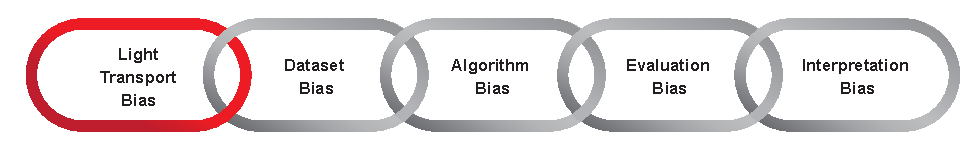
\includegraphics[width=\linewidth]{include/F_chain2.pdf}
    \caption{\textbf{The chain of biases in vision.} At the top of the chain lies the decision-making biases, which includes interpretation bias caused by the inappropriate analysis of results and evaluation bias caused by inappropriate benchmarks and statistical analyses used for evaluation. In the middle of the chain lies the computational biases, which includes algorithm bias caused by inappropriate machine-learned or software-embedded features and dataset bias caused by uneven distribution of training data. Finally, at the bottom of the chain lies the physical bias, which for vision systems is light transport bias caused by the physical laws and principles of sensing equipment. The focus of this section is highlighting the light transport bias in R-PPG.}
    \label{fig:chain_bias}
\end{figure}

\begin{figure}
    \centering
    \includegraphics[width=\linewidth]{include/fig-light-transport-skin.pdf}
    \caption{\textbf{Skin melanin fraction plays an important role when assessing physiological properties from human skin.} (a) The world map of skin tone of indigenous people shows skin coloration is strongly correlated with UV radiation levels. This suggests melanin pigementation, which determines skin tone, has a part in regulating the effects of radiation on the contents of blood vessels located in the dermis. (b) A two-layer skin model based on prior biorealistic rendering works is used to develop the light transport theory for R-PPG. The incident light ray attenuates through the epidermis. Following dermal reflection and another epidermal attenuation, the resultant ray properties are dependent on human physiological quantities. Source: Map is adapted from Jablonski \& Chaplin (2000).}
    \label{fig:light_transport_skin}
\end{figure}

In recent years, there has been a rising concern regarding the bias of vision-based systems \cite{brandao_age_2019,buolamwini_gender_2018,klare_face_2012,vangara_characterizing_2019}. A biased system or device is one that operates in a manner that disadvantages certain demographic groups and influences inequity. The important work of Nowara \textit{et al.} \cite{nowara_meta-analysis_2020} highlights the bias encompassing R-PPG technologies with respect to subject skin tone and gender, namely the poor performance for dark skin tones and women. To address this complex issue of bias, the computer vision community has rightly pointed out factors that include dataset bias, algorithmic bias, and decision-making bias. However, there is another type of bias that is less discussed: the bias encountered by the laws of physics. Vision-based systems, including R-PPG, rely on light-sensing cameras; however, the physics of light itself may involve bias. 

Kadambi \cite{kadambi_achieving_2021} highlights the various biases that may exist in medical devices, namely physical bias, computational bias, and interpretation bias. Figure~\ref{fig:chain_bias} extends this idea and outlines the chain of biases in vision-based systems. At the top of the chain lies the decision-making biases, which includes interpretation bias caused by the inappropriate analysis of results and evaluation bias caused by inappropriate benchmarks and statistical analyses used for evaluation. In the middle of the chain lies the computational biases, which includes algorithm bias caused by inappropriate machine-learned or software-embedded features and dataset bias caused by uneven distribution of training data. Finally, at the bottom of the chain lies the physical bias, which for vision systems is light transport bias caused by the physical laws and principles of sensing equipment. 

Light transport bias for medical devices is a rarely considered factor. Traditionally, medical devices rely on empirically determined calibration constants to estimate physiological parameters. In the case of pulse oximeters, the constants used do not account for variations in skin structure, including skin melanin fraction. However, Jablonski \& Chaplin \cite{jablonski_evolution_2000} concluded that one of the main roles of melanin pigmentation is the regulation of the effects of UV radiation on the contents of blood vessels located in the dermis. This conclusion was made after observing a high correlation between the skin tone of indigenous people around the world with absolute latitude and UV radiation, visually seen in Figure~\ref{fig:light_transport_skin}a. Therefore, by not accounting for the role of melanin or skin tone, pulse oximeters fail to calibrate for a key variable that affects skin light absorption and, consequently, blood oxygenation estimation. This fact has come to light recently with works highlighting the skin tone bias present in pulse oximeters \cite{sjoding_racial_2020}. 

In the following section, we establish a novel light transport theory for R-PPG that enables valuable insight into the origins of the skin tone bias. We will show that the signal strength reduces with increasing skin melanin content for all color channels, as intuitively expected. The decreasing signal strength leads us to an analysis of imaging noise, which is the major noise phenomenon at play in this case. Knowledge that the root of bias in R-PPG is due to light transport bias, which is exacerbated by imaging noise, leads us to a novel R-PPG algorithm described in Chapter~\ref{chap:methods} that significantly reduces the skin tone bias without fundamental changes to the hardware of the system. Beyond the light transport bias, this thesis also utilizes a new telemedicine-focused dataset that alleviates dataset bias, and highlights how previous R-PPG algorithms exhibit algorithmic bias. 

\section{Light Transport for R-PPG}

% \begin{figure}[t]
%     \centering
%     \includegraphics[height=3in]{include/fig_skin.pdf}
%     \caption{\textbf{A two-layer skin model used in prior biorealistic rendering works is used to develop the light transport theory for R-PPG.} The incident light ray attenuates through the epidermis. Following dermal reflection and another epidermal attenuation, the resultant ray properties are dependent on human physiological quantities.}
%     \label{fig:skin_model}
% \end{figure}

Plethysmographic estimation methods are enabled through the sensing of blood perfusion in the face. Specifically, the presence of varying volumes of blood under the skin manifest as minute changes in reflection properties of the overall skin system, as viewed by a camera. It is by identifying these changes that relevant physiological properties may be estimated. 

In order to set up a novel light transport theory for R-PPG, we utilize existing biorealistic graphical rendering models~\cite{krishnaswamy_biophysically_2004,igarashi_appearance_2007} and extend them for R-PPG signal generation. Figure~\ref{fig:light_transport_skin}b shows the skin model assumed for our computations, similar to~\cite{alotaibi_biophysical_2017}. Specifically, a two layer skin model is assumed. The incident light undergoes attenuation while passing through the epidermis, while it undergoes scattering driven reflection at the dermis. 

% \subsection{Epidermal Transmission}
We start with describing the epidermal transmission. Following the Beer-Lambert Law, 
\begin{equation} \label{eqn:T_epidermis}
    \mathbf{T_{epi}(\boldsymbol{\lambda})=e^{-\boldsymbol\mu_{a,epi}(\boldsymbol\lambda)}},
\end{equation}
Where $\mathbf{\boldsymbol\mu_{a,epi}(\boldsymbol\lambda)}$ is the absorption coefficient of the epidermis. Typically, this is modelled as a convex combination of skin tissue and melanin absorption,
\begin{equation} \label{eqn:mu_epidermis}
    \mathbf{\boldsymbol\mu_{a,epi}(\boldsymbol\lambda)=f_{mel}\boldsymbol\mu_{a,mel}(\boldsymbol\lambda)+(1-f_{mel})\boldsymbol\mu_{a,ski}(\boldsymbol\lambda)}.
\end{equation}

$\mathbf{\boldsymbol\mu_{a,ski}(\boldsymbol\lambda)}$, the skin tissue absorption coefficient, is a biological parameters which is known. $\mathbf{\boldsymbol\mu_{a,mel}(\boldsymbol\lambda)}$ may be defined as,
\begin{equation} \label{eqn:mu_melanin}
    \mathbf{\boldsymbol\mu_{a,mel}(\boldsymbol\lambda)=f_{eum}\boldsymbol\mu_{a,eum}(\boldsymbol\lambda)+(1-f_{eum})\boldsymbol\mu_{a,phm}(\boldsymbol\lambda)},
\end{equation}
Where ${\mathbf{\boldsymbol\mu_{a,eum}(\boldsymbol\lambda)}}$ is the absorption coefficient of eumelanin and $\mathbf{\boldsymbol\mu_{a,phm}(\boldsymbol\lambda)}$ is the absorption coefficient of pheomelanin, all biophysical known parameters. By combining Equations~\ref{eqn:T_epidermis}, \ref{eqn:mu_epidermis} and \ref{eqn:mu_melanin}, the epidermal transmission may be accurately modelled.

% \subsection{Dermal Reflection} 
We move towards describing the dermal reflection. This model follows the Kubelka-Munk theory for scattering-dependent reflection. Specifically, the fraction of reflected light, as a function of wavelength, is given by,
\begin{equation}
    \mathbf{R_{d}(\boldsymbol\lambda)=\frac{(1-\boldsymbol\beta(\boldsymbol\lambda))^2(e^{K(\boldsymbol\lambda)d_{der}}-e^{-K(\boldsymbol\lambda)d_{der}})}{(1+\boldsymbol\beta(\boldsymbol\lambda))^2e^{K(\boldsymbol\lambda)d_{der}}-(1-\boldsymbol\beta(\boldsymbol\lambda))^2e^{-K(\boldsymbol\lambda)d_{der}}}}
\end{equation}
Here, $\mathbf{\boldsymbol\beta(\boldsymbol\lambda)}$ and $\mathbf{K(\boldsymbol\lambda)}$ are deterministically related to $\mathbf{\boldsymbol\mu_{a,der}(\boldsymbol\lambda)}$ (dermal absorption coefficient) and $\mathbf{\boldsymbol\mu_{s,der}(\boldsymbol\lambda)}$ (reduced dermal scattering coefficient, known~\cite{anderson_optics_1981}). Similar to previously, the dermal absorption coefficient and the blood absorption coefficient are understood as convex combinations shown below:
\begin{equation}
    \mathbf{\boldsymbol\mu_{a,der}(\boldsymbol\lambda)=f_{bld}\boldsymbol\mu_{a,bld}(\boldsymbol\lambda)+(1-f_{bld})\boldsymbol\mu_{a,ski}(\boldsymbol\lambda)}
\end{equation}
\begin{equation}
    \mathbf{\boldsymbol\mu_{a,bld}(\boldsymbol\lambda)=f_{oxy}\boldsymbol\mu_{oxy}(\boldsymbol\lambda)+(1-f_{oxy})\boldsymbol\mu_{dox}(\boldsymbol\lambda)}
\end{equation}
Here, various factors include blood reflection, skin baseline reflection, oxygenated blood reflection and deoxygenated blood reflection respectively.

% \subsection{Overall Reflection} 
Given the expressions for epidermal transmission and dermal reflection, the expression for overall reflection is given by,
\begin{equation}
    \mathbf{R(\boldsymbol\lambda) = T{^2}_{epi}.R_{d}(\boldsymbol\lambda)}.
\end{equation}

Then, the overall intensity captured in channel $\mathbf{c}$ of the camera is given by,
\begin{equation}
    \mathbf{I_c=\boldsymbol\int_{\boldsymbol\lambda}E(\boldsymbol\lambda)S_{c}(\boldsymbol\lambda)R(\boldsymbol\lambda)d\boldsymbol\lambda},
\end{equation}
Where $\mathbf{E(\boldsymbol\lambda)}$ is the source spectral distribution and $\mathbf{S_{c}(\boldsymbol\lambda)}$ is the camera spectral response for channel $\mathbf{c}$.

\section{R-PPG Signal Strength} 

The R-PPG signal arises out of a variation in the blood volume fraction, $\mathbf{f_{bl}}$ under the skin. Our interest is in the signal strength across camera channels, $\boldsymbol\Sigma_{c}$, which can be defined as \textit{the maximum variation in the captured intensity}. Mathematically,
\begin{equation}
\begin{split}
    &\mathbf{\boldsymbol\Sigma_{c}=\boldsymbol\Delta I_c\boldsymbol\approx \Big|\frac{\boldsymbol\partial I_c}{\boldsymbol\partial f_{bl}}\Big|\cdot\boldsymbol\Delta f_{bl}}
\end{split}
\end{equation}
Since $\mathbf{R(\boldsymbol\lambda)}$ is the only term dependent on $\mathbf{f_{bl}}$,
\begin{equation}
\begin{split}
    &\mathbf{\boldsymbol\Sigma_{c}\boldsymbol\approx  \Big|\boldsymbol\int_{\boldsymbol\lambda}E(\boldsymbol\lambda)S_{c}(\boldsymbol\lambda)\frac{\boldsymbol\partial R}{\boldsymbol\partial f_{bl}}\Bigg|_{\overline{f_{bl}}} d\boldsymbol\lambda \Big| \cdot \boldsymbol\Delta f_{bl}},
\end{split}
\end{equation}
Where $\mathbf{\overline{f_{bl}}}$ is the average blood volume fraction, typically around $0.05$. This approximation holds true since $\mathbf{f_{bl}}$ only varies by a small amount, typically around $0.05$. 

This plethysmographic signal rides on top of the average skin tone color, given by
\begin{equation}
    \mathbf{\boldsymbol\Gamma_c=\boldsymbol\int_{\boldsymbol\lambda}E(\boldsymbol\lambda)S_{c}(\boldsymbol\lambda)R(\boldsymbol\lambda)\Big|_{\overline{f_{bl}}} d\boldsymbol\lambda}.
\end{equation}

Since, $\boldsymbol\Sigma_{c}$ and $\boldsymbol\Gamma_{c}$ are both dependent on $\mathbf{f_{mel}}$, as a result of the dependence of $\mathbf{R(\cdot)}$ on the same, we refer to these as $\mathbf{\boldsymbol\Sigma(f_{mel})}$ and $\mathbf{\boldsymbol\Gamma(f_{mel})}$ subsequently.

% {\color{red} 
% \begin{enumerate}
%     \item Add parameter values used/the source paper for the same, for reproducability.
%     \item Not clear what you mean by average camera response function. Also, where did we get the average response function from? We should cite our sources for reproducability. Same goes for light source characteristics.
% \end{enumerate}
% }

\begin{figure}[t]
    \centering
    \includegraphics[width=\linewidth]{include/fig_strength_dB.pdf}
    \caption{\textbf{The R-PPG signal strength is critically related to skin melanin fraction as well as scene lighting.} As opposed to previously accepted fact, the three channels may contain differing amounts of signal information, depending on regime of operation.}
    \label{fig:signal_strength}
\end{figure}

Figure~\ref{fig:signal_strength} shows the signal strength plots for the three camera color channels, across lighting conditions. We use average camera response functions $\mathbf{S_c(\boldsymbol\lambda)}$ to identify responsiveness of each of the channels to incident light. We also generate signal strength across common light source characteristics. These plots provide incisive detail: the overall signal strength decays with increasing skin melanin fraction. Additionally, while previous works~\cite{verkruysse_remote_2008,haan_robust_2013,wang_algorithmic_2017} have empirically determined that the green channel holds maximum R-PPG signal information, we show for the first time that this in-fact heavily depends on melanin fraction and scene lighting. While the green channel is dominant for light skin tones, for darker skin tones, the channel-wise signal strength depends significantly on lighting conditions and skin tone.

\section{Effect of Imaging Noise on R-PPG}\label{sec:effect_noise_RPPG}

The goal of this subsection is to understand the relationship between imaging noise and R-PPG algorithm estimation. Imaging noise refers to the inherent noise that arises due to the image capture process in a commercial camera. This arises due to various effects related to photon arrival processes, thermal noise in electronics and the quantization noise associated with digitally capturing images \cite{hasinoff_noise-optimal_2010}. For
pixels below the saturation level, the noise can be modelled as follows: 
\begin{equation} \label{eqn:imaging_noise_model}
    \sigma_{pixel}^2 = \frac{\Phi t}{g^2} + \frac{\sigma_{r}^2}{g^2} + \sigma_{q}^2
\end{equation}
where $\Phi$ is the radiant power of light collect, $t$ is the exposure time, $g$ is the sensor gain (a constant for a given image), and $\sigma_r$ and $\sigma_q$ are camera noie parameters (also constant). 

Using this noise model, we can the estimate the entire R-PPG signal to noise ratio (SNR) for a pixel of a particular intensity and color channel $c$ as follows:
\begin{equation} \label{eqn:SNR_rPPG}
    \mathbf{SNR_c} = \frac{\mathbf{\boldsymbol\Sigma_{c}}t}{\sqrt{\frac{\mathbf{\boldsymbol\Gamma_{c}}t}{g^2} + \frac{\sigma_{r}^2}{g^2} + \sigma_{q}^2}}
\end{equation}
Here, we assume that the radiant power of light collected $\Phi$ is equal to the average skin tone color. 

\begin{figure}[t]
    \centering
    \includegraphics[width=\linewidth]{include/fig_SNR_dB.pdf}
    \caption{\textbf{The R-PPG SNR drastically worsens with increasing skin melanin fraction.} As expected, the R-PPG SNR reduces by orders of magnitude as the skin melanin fraction increases. Therefore, mitigating the skin tone bias present in R-PPG will require strategies that emphasize capturing more signal and reducing noise.}
    \label{fig:SNR_theory}
\end{figure}

Figure~\ref{fig:SNR_theory} shows the R-PPG SNR plots for the three camera color channels, across lighting conditions. These observations are similar to those of the R-PPG signal strength, namely that the SNR decays with increasing skin melanin fraction. This leads us to the following inferences: 
\begin{enumerate}[label=(\roman*)]
    \item \textbf{Imaging noise creates skin tone bias (and lighting bias):} The performance gap across skin tones, as well as across lighting differences, can be understood in terms of imaging noise. Darker skin regions have lower signal strength that manifest as lower pixel value changes in the video. This results in poorer SNRs. Note that this inference also holds true for shadowed regions, thereby extending this analysis towards understanding lighting bias.
    \item \textbf{Imaging noise and specular reflections degrade the R-PPG signal:} Imaging noise, coupled with specular highlights due to lighting, are the major contributing factors to signal degradation. The corruption due to imaging noise depends on signal intensity. The corruption due to specular highlights depends on lighting conditions- regions with strong specular highlights have relatively lower PPG signal information. Combating the highlighted biases in existing R-PPG would therefore involve a principled approach towards reduction of the above highlighted imaging noise and specular highlight removal. Note that specular highlight removal, in addition to reducing lighting related biases, also indirectly affects skin tone bias: darker skin subjects are worse affected by these interferences, since the intensity difference between the signal and the highlight is much more. 
\end{enumerate}

We conclude that addressing this low-level light transport bias must occur in order to drastically mitigate the skin tone bias present in R-PPG. Biases higher up the chain of biases, such as algorithmic or dataset bias, must also be addressed, but may not necessarily overcome this fundamental physics-based problem. Therefore, image and signal processing strategies to increase signal capture and reduce noise may drastically improve performance for darker skin tone subjects as opposed to modifications to signal inference algorithms. With the inferences from this chapter in mind, we motivate our novel R-PPG algorithm outlined in the following Methods section.

